\documentclass[10pt,a4paper]{article} 
\usepackage[utf8]{inputenc}
\usepackage{amsmath}
\usepackage{amsfonts}
\usepackage{amssymb}
\usepackage{graphicx}
\usepackage{epstopdf}
\usepackage[ngerman]{babel}
\usepackage[ngerman]{translator}
\usepackage{listings}
\usepackage[colorlinks=true,
        linkcolor=black,
        citecolor=black,
        filecolor=black,
        pagecolor=black,
        urlcolor=black,
        bookmarks=true,
        bookmarksopen=true,
        bookmarksopenlevel=3,
        plainpages=false,
        pdfpagelabels=true]{hyperref}


%Paket laden
\usepackage[
	nonumberlist, %keine Seitenzahlen anzeigen
	acronym,      %ein Abkürzungsverzeichnis erstellen
	toc,          %Einträge im Inhaltsverzeichnis
	section]      %im Inhaltsverzeichnis auf section-Ebene erscheinen
	{glossaries}
\usepackage{pdfpages}


\parindent 0pt
\pagestyle{headings}

%\let\oldsection\section
%\renewcommand{\section}{\newpage \oldsection}

\title{
	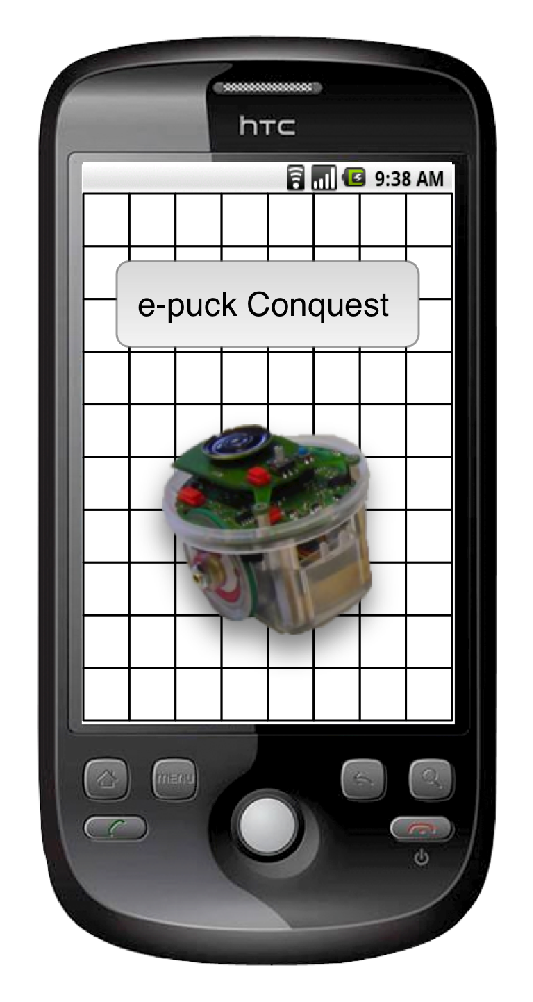
\includegraphics[height=10cm]{logo.eps} \\
%	\vspace{1cm}
	Validierungsbericht
}
\author{
            \begin{tabular}[r]{*{3}{|c|}}
	\hline
	Phase & Verantwortlicher & E-Mail \\
	\hline \hline
	Pflichtenheft & Florian Lorenz & lorenz@fim.uni-passau.de \\
	\hline
	Entwurf & Andreas Wilhelm &  wilhelma@fim.uni-passau.de \\
	\hline
	Spezifikation & Andreas Poxrucker & poxrucke@fim.uni-passau.de \\
	\hline
	Implementierung & Martin Freund & freund@fim.uni-passau.de \\
	\hline
	Validierung & Florian Bürchner & buerchne@fim.uni-passau.de \\
	\hline
	Präsentation & Max Binder & binder@fim.uni-passau.de \\
	\hline
	\end{tabular}
}

\date{21. Januar 2011}
	
	
\begin{document}

	\maketitle
	\newpage
	\tableofcontents
	\newpage

	\begin{abstract}
		Dieses Dokument soll einen Überblick über ...
	\end{abstract}	

	\section{Globale Testszenarien und Testfälle}
		\subsection{Pflichtenheft Testfälle}
			\subsubsection{/T50/ Kalibrierung}
			Nach nicht ordnungsgemäßer Kalibrierung beginnen die Außen-LEDs nacheinander zu leuchten (/F180/).
			
			\subsubsection{/T60/ Linienerkennung}
			Der e-puck wird im Betrieb entlang einer Linie aufgestellt und folgt dieser in Richtung der
			Liniensensoren (/F100/).
			
			\subsubsection{/T70/ Bluetooth-Scan}
			Mehrere e-puck-Roboter werden auf dem Spielfeld platziert und eingeschaltet. Nach der Initialisierungsphase
			sollen sämtliche Teilnehmer auf dem Smartphone erkannt werden (/F200/).
			
			\subsubsection{/T80/ Broadcast-Test}
			Gemäß /T70/ werden alle verbindungsbereiten e-puck Roboter auf dem Suchdialog des Smartphones
			angezeigt. Es wird ein Roboter ausgewählt, alle im Netzwerk befindlichen Teilnehmer werden im Dropdown-Steuerelement
			aufgelistet  (/F50/, /F60/, /F65/, /F70/, /F205/, /F210/).
			
			\subsubsection{/T90/ Knotenanalyse und manuelle Steuerung per On-Screen-Joystick}
			Der Roboter wird gemäß /T60/ aufgestellt. Durch manuelle Steuerung per On-Screen-Joystick muss der
			Benutzer auf allen Knotentypen die möglichen Fahrtrichtungen testen. Nur gültige Richtungen
			dürfen vom Roboter befahren werden (/F80/, /F110/, /F220/, /F270/).
			
			\subsubsection{/T100/ Steuerung der Fahrtgeschwindigkeit}
			Dieser Test konnte aufgrund der ge\"anderten Funktionalit\"aten nicht durchgef\"uhrt werden.
			
			\subsubsection{/T110/ Steuerung per Beschleunigungssensor}
			Der Test wird analog zu /T80/ durchgeführt, wobei als Steuerungsmethode der Beschleunigungssensor
			verwendet wird (/F280/).
			
			\subsubsection{/T120/ Erkundungstest}
			Mehrere e-puck Roboter werden auf entsprechende Startpositionen innerhalb des Spielfelds gesetzt und
			eingeschaltet. Ziel des Testszenarios ist die vollständige Erkundung durch effiziente Zusammenarbeit der Teilnehmer.
			Falls die Roboter nach Abschluss auf die Startpositionen zurückkehren und die Karte auf dem Smartphone dargestellt
			wird, ist der Testfall erfolgreich (/F90/, /F120/, /F130/, /F135/, /F140/,
			/F150/, /F155/, /F160/, /F190W/, /F230/, /F320/, /F330/).
			
			\subsubsection{/T130/ Erweiterter Steuerungstest}
			Der Benutzer wählt nach der Lokalisierung von mindestens zwei Roboter einen per Dropdown-Steuerelement aus.
			Anschließend wird die Steuerung über beide Steuerungsarten (/F270/, /F280/) durchgeführt. Im nächsten
			Schritt wird eine anderer Roboter gewählt und die Steuerung mit diesem geprüft (/F290/, /F300/, /F310/).
			
			\subsubsection{/T140W/ Speichern der Kartendaten}
			Nachdem eine Kartenansicht auf dem Smartphone verfügbar ist, speichert der Benutzer die Kartendaten ab (/F250W/).
			
			\subsubsection{/T150W/ Laden der Kartendaten}
			Nachdem Kartendaten auf dem Smartphone gespeichert wurden (/T120W/), lädt der Benutzer diese.
			Daraufhin wird die entsprechende Karte angezeigt (/F260W/).
			
			\subsubsection{/T160W/ Test von globaler Lokalisierung}
			Dieser Test konnte aufgrund der ge\"anderten Funktionalit\"aten nicht durchgef\"uhrt werden.
			
			\subsubsection{/T170W/ Test der Zoomfunktionalit\"at}
			Dieser Test konnte aufgrund der ge\"anderten Funktionalit\"aten nicht durchgef\"uhrt werden.
		
		\subsection{weitere Testfälle}
					\subsubsection{Test der Autoskalierung}
					Es werden nacheinander zwei unterschiedlich gro\ss e Karten mittels Import-Funktion (/F260W/) geladen. Beide Karten
					werden nun autoskaliert und vollst\"andig angezeigt.
					\subsubsection{Test der Karten\"uberpr\"ufung auf G\"ultigkeit}
					Es werden ung\"ultige Karten erstellt und nacheinander geladen. Es wird eine Meldung ausgegeben, dass die Karte nicht g\"ultig ist.
	
	\section{Unit Tests}
		\subsection{Android Anwendung}
		
			\subsubsection{GridMap}
			\begin{itemize}
				\item \texttt{testInsertNode()} Ein neuer Knoten wird erstellt und in die GridMap eingefügt. Anschließend wird die GridMap in eine Liste umgewandelt und deren Größe 							abgefragt, um sicherzustellen, dass der Knoten eingefügt wurde.
				\item \texttt{testFrontierNodeRightT()} Ein neuer Knoten wird erstellt und in die GridMap eingefügt. Anschließend wird durch die GridMap eine Liste mit Frontierknoten 							erstellt und überprüft, ob drei Frontierknoten eingefügt wurden.
				\item \texttt{testFrontierNodeLeftT()} Ein neuer Knoten wird erstellt und in die GridMap eingefügt. Anschließend wird durch die GridMap eine Liste mit Frontierknoten 							erstellt und überprüft, ob drei Frontierknoten eingefügt wurden.
				\item \texttt{testFrontierNodeTopT()} Ein neuer Knoten wird erstellt und in die GridMap eingefügt. Anschließend wird durch die GridMap eine Liste mit Frontierknoten 							erstellt und überprüft, ob drei Frontierknoten eingefügt wurden.
				\item \texttt{testFrontierNodeBottomT()} Ein neuer Knoten wird erstellt und in die GridMap eingefügt. Anschließend wird durch die GridMap eine Liste mit Frontierknoten 							erstellt und überprüft, ob drei Frontierknoten eingefügt wurden.
				\item \texttt{testFrontierNodeCross()} Ein neuer Knoten wird erstellt und in die GridMap eingefügt. Anschließend wird durch die GridMap eine Liste mit Frontierknoten 							erstellt und überprüft, ob vier Frontierknoten eingefügt wurden.
				\item \texttt{testFrontierNodeBottomRightEdge()} Ein neuer Knoten wird erstellt und in die GridMap eingefügt. Anschließend wird durch die GridMap eine Liste mit 								Frontierknoten erstellt und überprüft, ob zwei Frontierknoten eingefügt wurden.
				\item \texttt{testFrontierNodeBottomLeftEdge()} Ein neuer Knoten wird erstellt und in die GridMap eingefügt. Anschließend wird durch die GridMap eine Liste mit 								Frontierknoten erstellt und überprüft, ob zwei Frontierknoten eingefügt wurden.
				\item \texttt{testFrontierNodeTopRightEdge()} Ein neuer Knoten wird erstellt und in die GridMap eingefügt. Anschließend wird durch die GridMap eine Liste mit 									Frontierknoten erstellt und überprüft, ob zwei Frontierknoten eingefügt wurden.
				\item \texttt{testFrontierNodeTopLeftEdge()} Ein neuer Knoten wird erstellt und in die GridMap eingefügt. Anschließend wird durch die GridMap eine Liste mit 									Frontierknoten erstellt und überprüft, ob zwei Frontierknoten eingefügt wurden.
				\item \texttt{testUpdateNode()} Es werden zwei neue Knoten erstellt und die GridMap eingefügt. Der zuletzt Eingefügte wird abgerufen und sein Knotentyp überprüft. Außerdem 					wird durch die GridMap erneut eine Liste mit Frontierknoten erstellt und deren Größe, die abhängig von der Wahl der Knotentypen ist, überprüft.
				\item \texttt{testMapBorders()} Es werden vier neue Knoten erstellt und in die GridMap eingefügt. Je nach Wahl der Koordinaten dieser Knoten wird hier die Größe des 							Spielfeldes überprüft. Es werden vier Werte verglichen, der minimale x Wert, der maximale x Wert, der minimale y Wert und der maximale y Wert.
				\item \texttt{testSerialieMapInString()} Ein neuer Knoten wird erstellt und in die GridMap eingefügt. Anschließend wird die serialisiert und in einem String Array 								gespeichert. Dieses Array beinhaltet nun den x, den y Wert und den Knotentyp der zuvor eingefügten Knoten, in genau dieser Reihenfolge. Es wird überprüft, ob sich diese Werte 				entsprechen.
			\end{itemize}
			
			\subsubsection{Behaviour}
			\begin{itemize}
				\item \texttt{testExploreBehaviour()} 
			\end{itemize}
			
			\subsubsection{ComManager}
			\begin{itemize}
				\item \texttt{testAddClientAndSend()}
				\item \texttt{testRemoveClient()}
			\end{itemize}
			
			\subsubsection{AStarPathFinder}
			\begin{itemize}
				\item \texttt{testFindPuckMapNodeMapNodeArray()} 
			\end{itemize}
			
			\subsubsection{Handler}
			\begin{itemize}
				\item \texttt{testSimTurnHandler()} Es wird eine neue Nachricht erzeugt im verwendeten Nachrichtenformat (32 Byte Array) erzeugt.
				Die ersten beiden Bytes der Nachricht (Nachrichtenheader) werden auf REQUEST\_TURN gesetzt. Anschließend wird mit dem Array ein neuer
				VirtualPuckRequest erzeugt und an den Handler weitergegeben.
				Der Test ist bestanden, wenn der Handler die Nachricht anhand des Nachrichtenheaders erkennt.
				\item \texttt{testSimStatusHandler()} Es wird eine neue Nachricht erzeugt im verwendeten Nachrichtenformat (32 Byte Array) erzeugt.
				Die ersten beiden Bytes der Nachricht (Nachrichtenheader) werden auf REQUEST\_STATUS gesetzt. Anschließend wird mit dem Array ein
				neuer VirtualPuckRequest erzeugt und an den Handler weitergegeben.
				Der Test ist bestanden, wenn der Handler die Nachricht anhand des Nachrichtenheaders erkennt.
				\item \texttt{testSimSpeedHandler()} Es wird eine neue Nachricht erzeugt im verwendeten Nachrichtenformat (32 Byte Array) erzeugt.
				Die ersten beiden Bytes der Nachricht (Nachrichtenheader) werden auf REQUEST\_SPEED gesetzt. Anschließend wird mit dem Array ein
				neuer VirtualPuckRequest erzeugt und an den Handler weitergegeben.
				Der Test ist bestanden, wenn der Handler die Nachricht anhand des Nachrichtenheaders erkennt.
				\item \texttt{testSimResetHandler()} Es wird eine neue Nachricht erzeugt im verwendeten Nachrichtenformat (32 Byte Array) erzeugt.
				Die ersten beiden Bytes der Nachricht (Nachrichtenheader) werden auf REQUEST\_RESET gesetzt. Anschließend wird mit dem Array ein neuer
				VirtualPuckRequest erzeugt und an den Handler weitergegeben.
				Der Test ist bestanden, wenn der Handler die Nachricht anhand des Nachrichtenheaders erkennt.
				\item \texttt{testSimMoveHandler()} Es wird eine neue Nachricht erzeugt im verwendeten Nachrichtenformat (32 Byte Array) erzeugt.
				Die ersten beiden Bytes der Nachricht (Nachrichtenheader) werden auf REQUEST\_MOVE gesetzt. Anschließend wird mit dem Array ein neuer
				VirtualPuckRequest erzeugt und an den Handler weitergegeben.
				Der Test ist bestanden, wenn der Handler die Nachricht anhand des Nachrichtenheaders erkennt.
				\item \texttt{testSimLEDHandler()} Es wird eine neue Nachricht erzeugt im verwendeten Nachrichtenformat (32 Byte Array) erzeugt.
				Die ersten beiden Bytes der Nachricht (Nachrichtenheader) werden auf REQUEST\_LED gesetzt. Anschließend wird mit dem Array ein neuer
				VirtualPuckRequest erzeugt und an den Handler weitergegeben.
				Der Test ist bestanden, wenn der Handler die Nachricht anhand des Nachrichtenheaders erkennt.
				\item \texttt{testPuckStatusHandler()} Es wird eine neue Nachricht erzeugt im verwendeten Nachrichtenformat (32 Byte Array) erzeugt.
				Die ersten beiden Bytes der Nachricht (Nachrichtenheader) werden auf RES\_STATUS gesetzt. Anschließend wird mit dem Array ein
				neuer PuckRequest erzeugt und an den Handler weitergegeben.
				Der Test ist bestanden, wenn der Handler die Nachricht anhand des Nachrichtenheaders erkennt.
				\item \texttt{testPuckRejectHandler()} Es wird eine neue Nachricht erzeugt im verwendeten Nachrichtenformat (32 Byte Array) erzeugt.
				Die ersten beiden Bytes der Nachricht (Nachrichtenheader) werden auf RES\_REJECT gesetzt. Anschließend wird mit dem Array ein
				neuer PuckRequest erzeugt und an den Handler weitergegeben.
				Der Test ist bestanden, wenn der Handler die Nachricht anhand des Nachrichtenheaders erkennt.
				\item \texttt{testPuckOkHandler()} Es wird eine neue Nachricht erzeugt im verwendeten Nachrichtenformat (32 Byte Array) erzeugt.
				Die ersten beiden Bytes der Nachricht (Nachrichtenheader) werden auf RES\_OK gesetzt. Anschließend wird mit dem Array ein
				neuer PuckRequest erzeugt und an den Handler weitergegeben.
				Der Test ist bestanden, wenn der Handler die Nachricht anhand des Nachrichtenheaders erkennt.
				\item \texttt{testPuckNodeHitHandler()} Es wird eine neue Nachricht erzeugt im verwendeten Nachrichtenformat (32 Byte Array) erzeugt.
				Die ersten beiden Bytes der Nachricht (Nachrichtenheader) werden auf RES\_HIT\_NODE gesetzt. Anschließend wird mit dem Array ein
				neuer PuckRequest erzeugt und an den Handler weitergegeben.
				Der Test ist bestanden, wenn der Handler die Nachricht anhand des Nachrichtenheaders erkennt.
				\item \texttt{testPuckCollisionHandler()} Es wird eine neue Nachricht erzeugt im verwendeten Nachrichtenformat (32 Byte Array)
				erzeugt. Die ersten beiden Bytes der Nachricht (Nachrichtenheader) werden auf RES\_COLLISION gesetzt. Anschließend wird mit dem Array
				ein neuer PuckRequest erzeugt und an den Handler weitergegeben.
				Der Test ist bestanden, wenn der Handler die Nachricht anhand des Nachrichtenheaders erkennt.
				\item \texttt{testPuckAbyssHandler()} Es wird eine neue Nachricht erzeugt im verwendeten Nachrichtenformat (32 Byte Array) erzeugt.
				Die ersten beiden Bytes der Nachricht (Nachrichtenheader) werden auf RES\_ABYSS gesetzt. Anschließend wird mit dem Array ein
				neuer PuckRequest erzeugt und an den Handler weitergegeben.
				Der Test ist bestanden, wenn der Handler die Nachricht anhand des Nachrichtenheaders erkennt.
				\item \texttt{testFailureRequestHandler()} Es wird eine neue FailureRequest-Nachricht erstellt und an den Handler übergeben. Der Test
				ist bestanden, wenn der Handler die Nachricht anhand des Nachrichtentyps erkennt.
				\item \texttt{testDriveRequestHandler()} Es wird eine neue DriveRequest-Nachricht erstellt und an den Handler übergeben. Der Test
				ist bestanden, wenn der Handler die Nachricht anhand des Nachrichtentyps erkennt.
				\item \texttt{testControlledRequestHandler()} Es wird eine neue ControlledRequest-Nachricht erstellt und an den Handler übergeben.
				Der Test ist bestanden, wenn der Handler die Nachricht anhand des Nachrichtentyps erkennt.
				\item \texttt{testCollisionRequestHandler()} Es wird eine neue CollisionRequest-Nachricht erstellt und an den Handler übergeben. Der
				Test ist bestanden, wenn der Handler die Nachricht anhand des Nachrichtentyps erkennt.
			\end{itemize}
		
		\subsection{e-puck Firmware}
		
			\subsubsection{Ringpuffer}
	
	\section{Blackbox Tests}
		\subsection{Simulator}
			Es wird eine Karte erstellt und im Simulator geladen. Anschlie\ss end wird eine Erkundung mit mehreren e-puck Robotern durchgef\"uhrt. Nach erfolgreicher
			Erkundung fahren die virtuellen Roboter auf ihre Ausgangsposition zur\"uck.
		\subsection{Mehrfach \"uberfahrene Knoten}
			Es wird eine Karte erstellt, die ein Roboter nicht abfahren kann, ohne einen Knoten mehrfach zu befahren. Die Erkundung wird dann mit mehreren Roboter 
 			gestartet und gepr\"uft, ob sich ein Knoten, wenn er mehrfach \"uberfahren worden ist verf\"arbt.
		\subsection{Steuerung}
			Nach erfolgreichem Verbindungsaufbau eines e-puck Roboters mit dem Smartphone wird zum Dialog \textit{Steer} gewechselt und der Roboter in alle vier
			Richtungen gesteuert. Der Vorgang wird mit der zweiten Steuerungsart wiederholt.		
		\subsection{Korrektes Anzeigen aller Schaltfl\"achen und der Karte}
			Es werden g\"ultige Karten erstellt und nacheinander geladen und gepr\"uft, ob sie korrekt dargestellt werden. Beim Verbinden mit den e-puck Robotern werden 
			nacheinander alle angezeigten Roboter an- und wieder abge\"ahlt. Diese m\"ussen farblich jeweils hervorgehoben werden. Anschlie\ss end wird zum Dialog 
			\textit{Steer} gewechselt und jeder Button f\"ur die Richtungen nacheinander gedr\"uckt und validiert, ob die jeweilige Auswahl hervorgehoben wird.
		\subsection{Men\"uf\"uhrung}
			Von jeder Activity wird \"uber das Men\"u zu allen anderen erreichbaren Dialogen gewechselt.
		\begin{figure}[htbp]
		\centering
			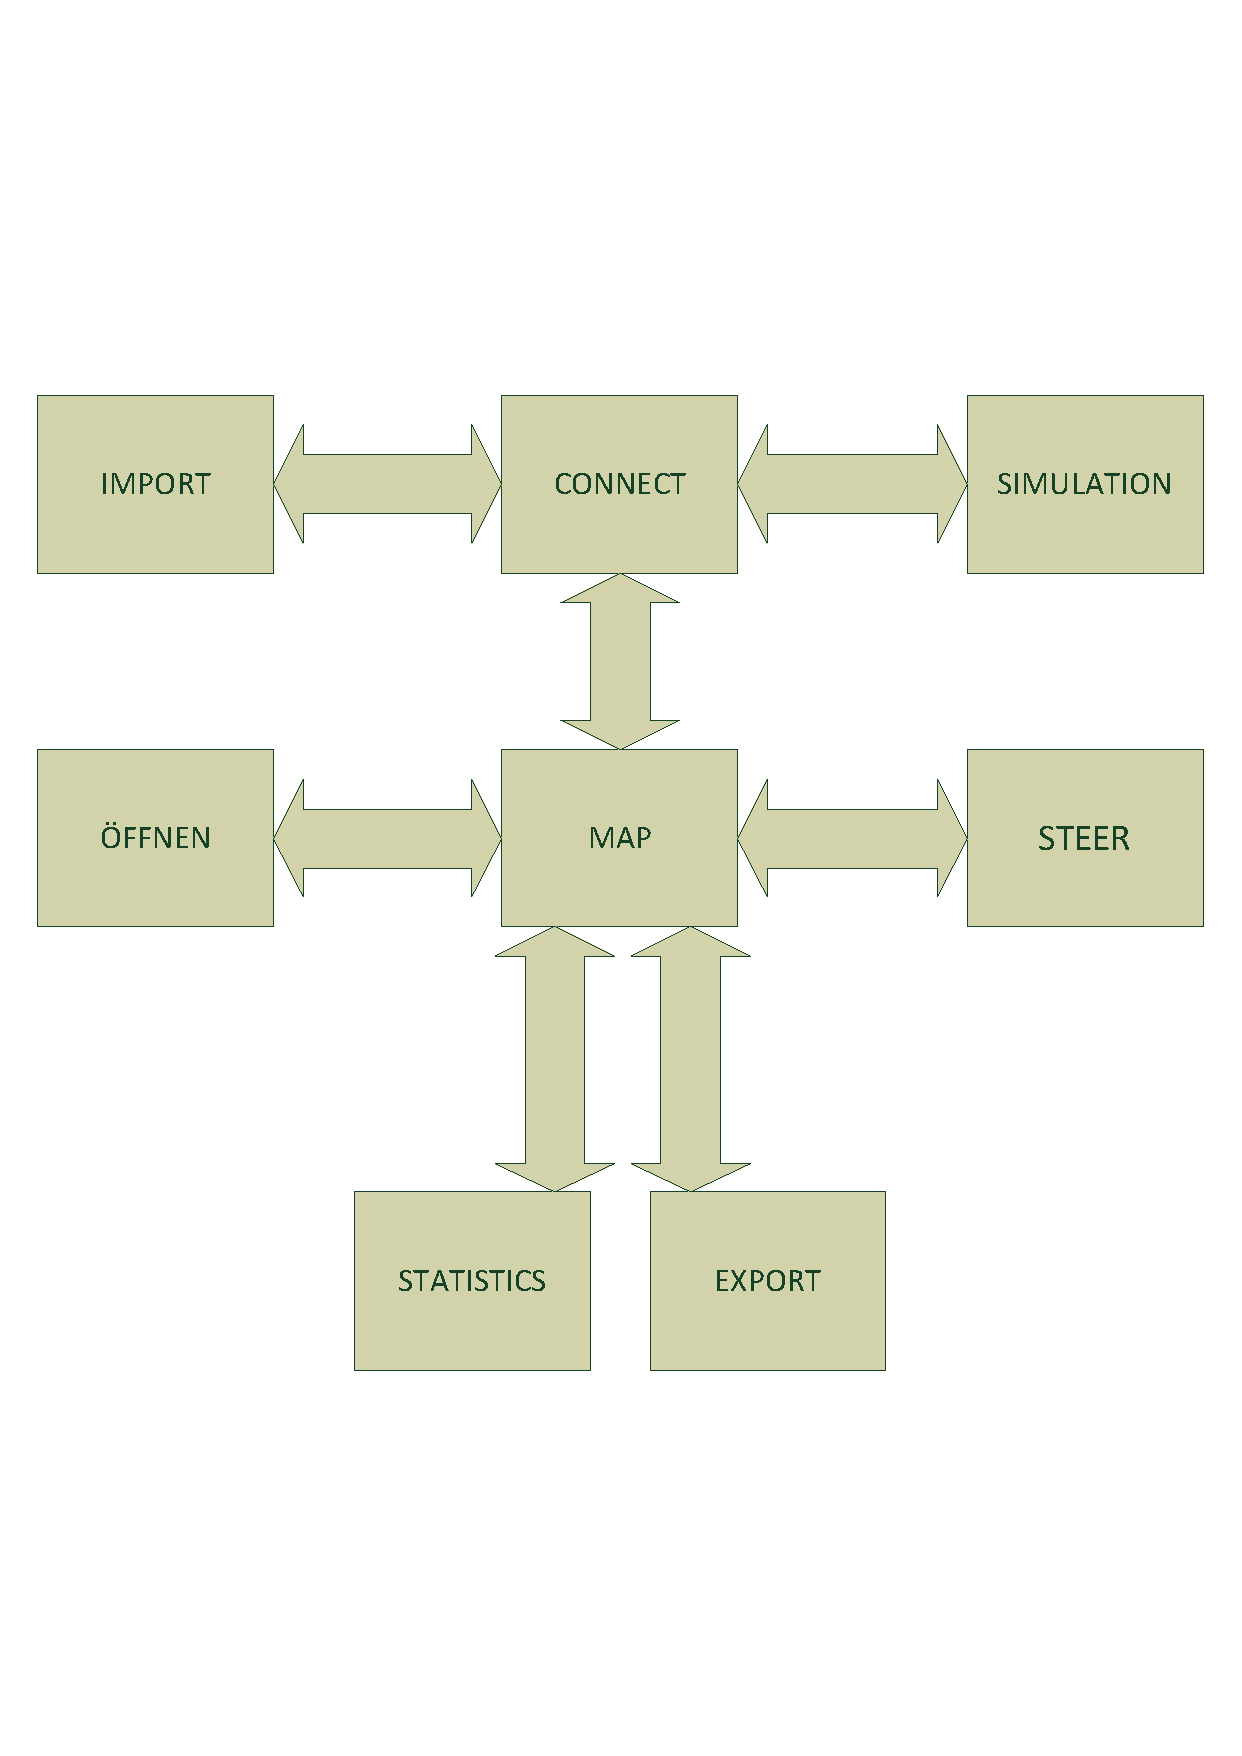
\includegraphics[width = 6cm]{images/Zeichnung1}
			\caption{Men\"uf\"uhrung}
		\end{figure}
		
	\section{kontrollflussorientierte Testverfahren}

				 			
\end{document}
